\chapter{Transferability of Interatomic Potentials}
\label{section:transferabilityappendix}


\section{Sheng Aluminium Potential}
\label{section:alshengxfer}

\subsection{FCC Structure}

The EAMPA code was used to compute both the Birch-Murnaghan and Rose-Vinet equations of state using the known values for Aluminium and the Sheng Al potential\cite{shengeamonline}.  
 
\begin{figure}
  \begin{center}
    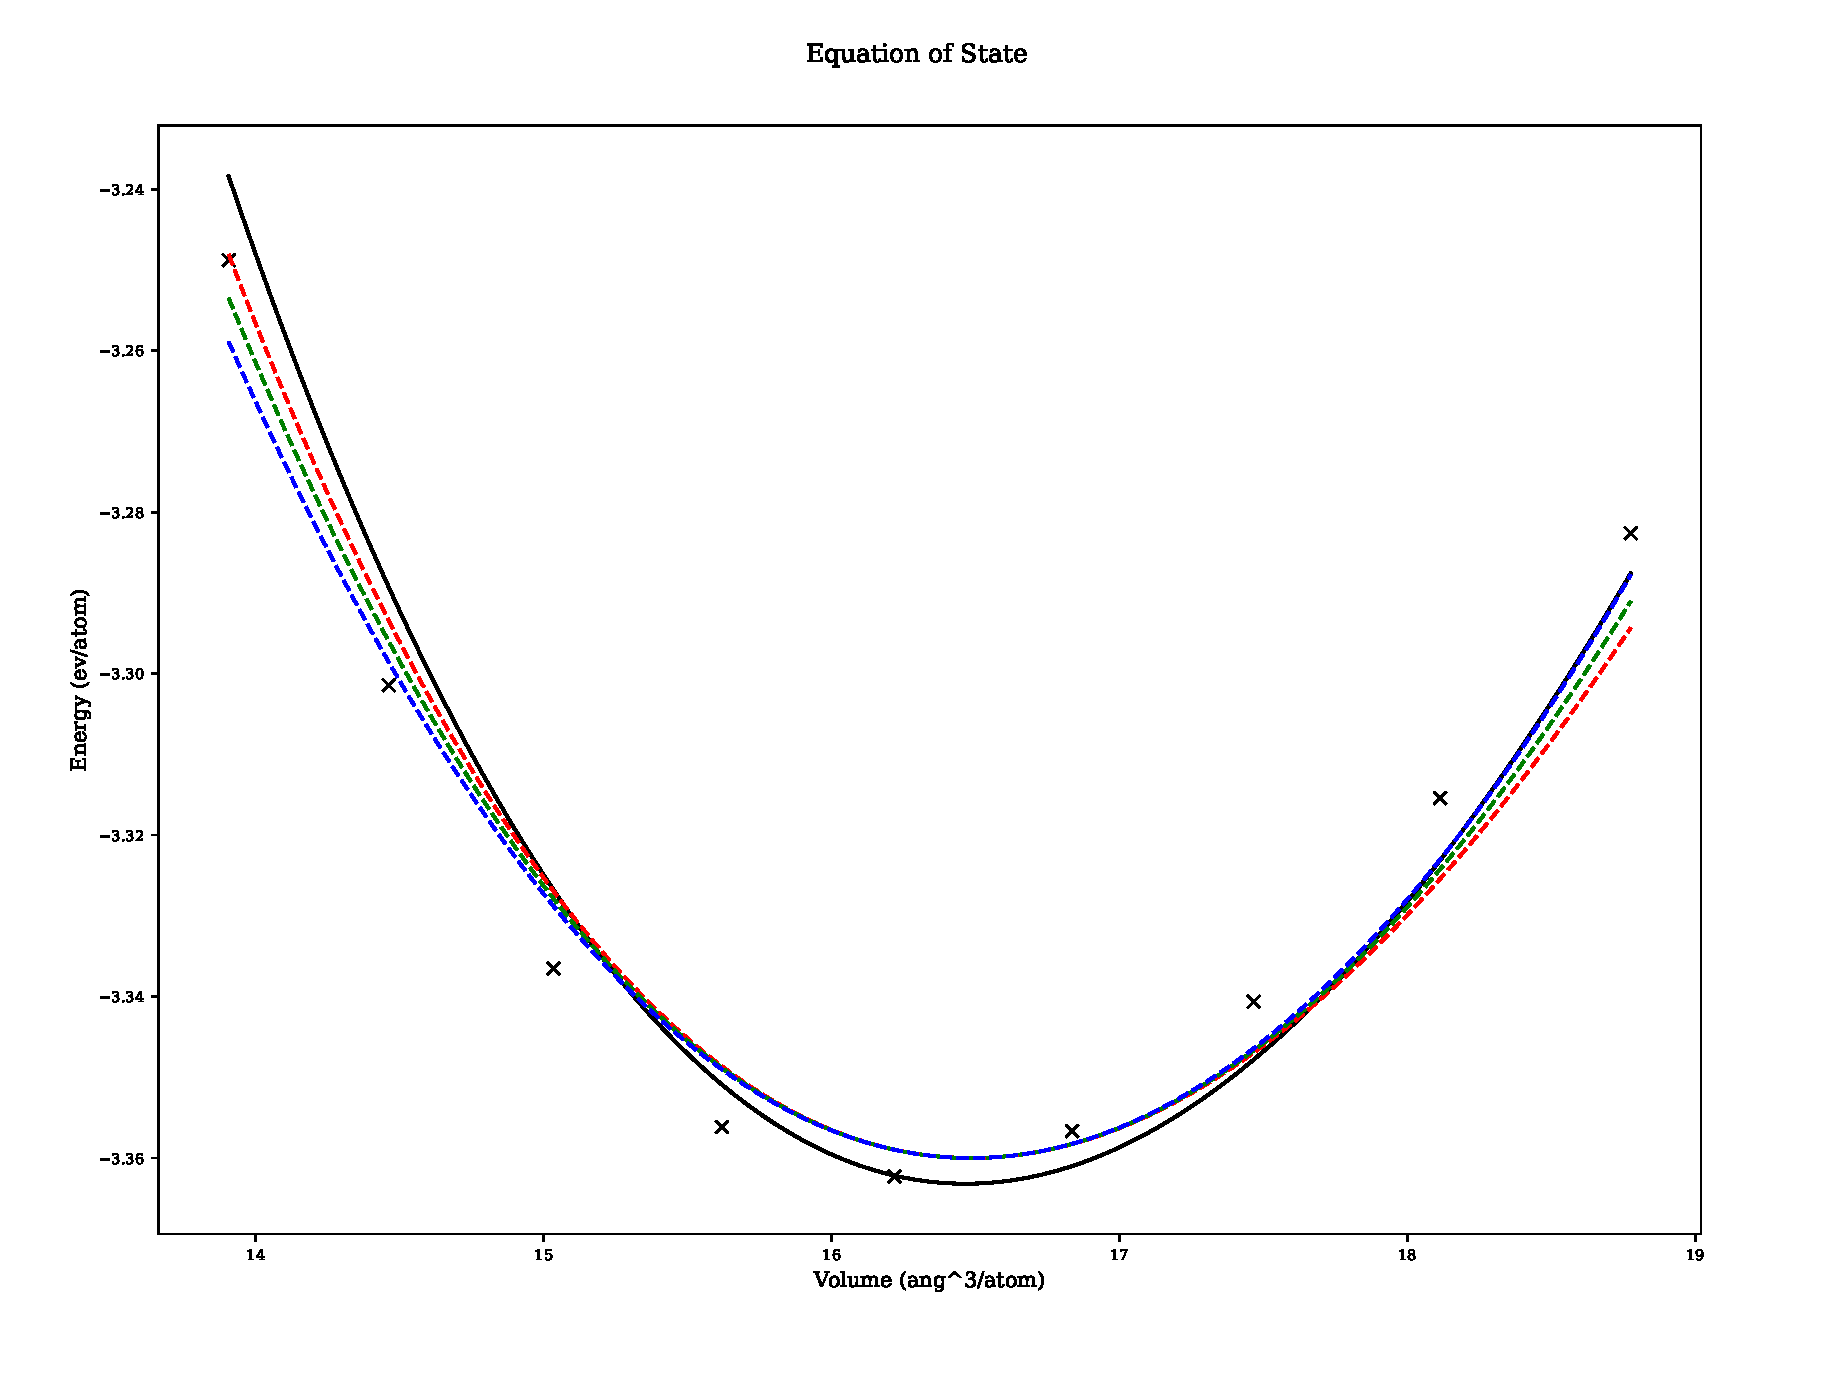
\includegraphics[width=0.6\linewidth]{appendix/transferability/transferability/Al_sheng/equation_of_state_bp_fcc.eps}
  \end{center}
	\caption{Birch Murnaghan equation of state for FCC Aluminium - comparison of experimental data to the Sheng Al potential}
	\label{fig:shengalfccbm}
\end{figure}

\begin{figure}
  \begin{center}
    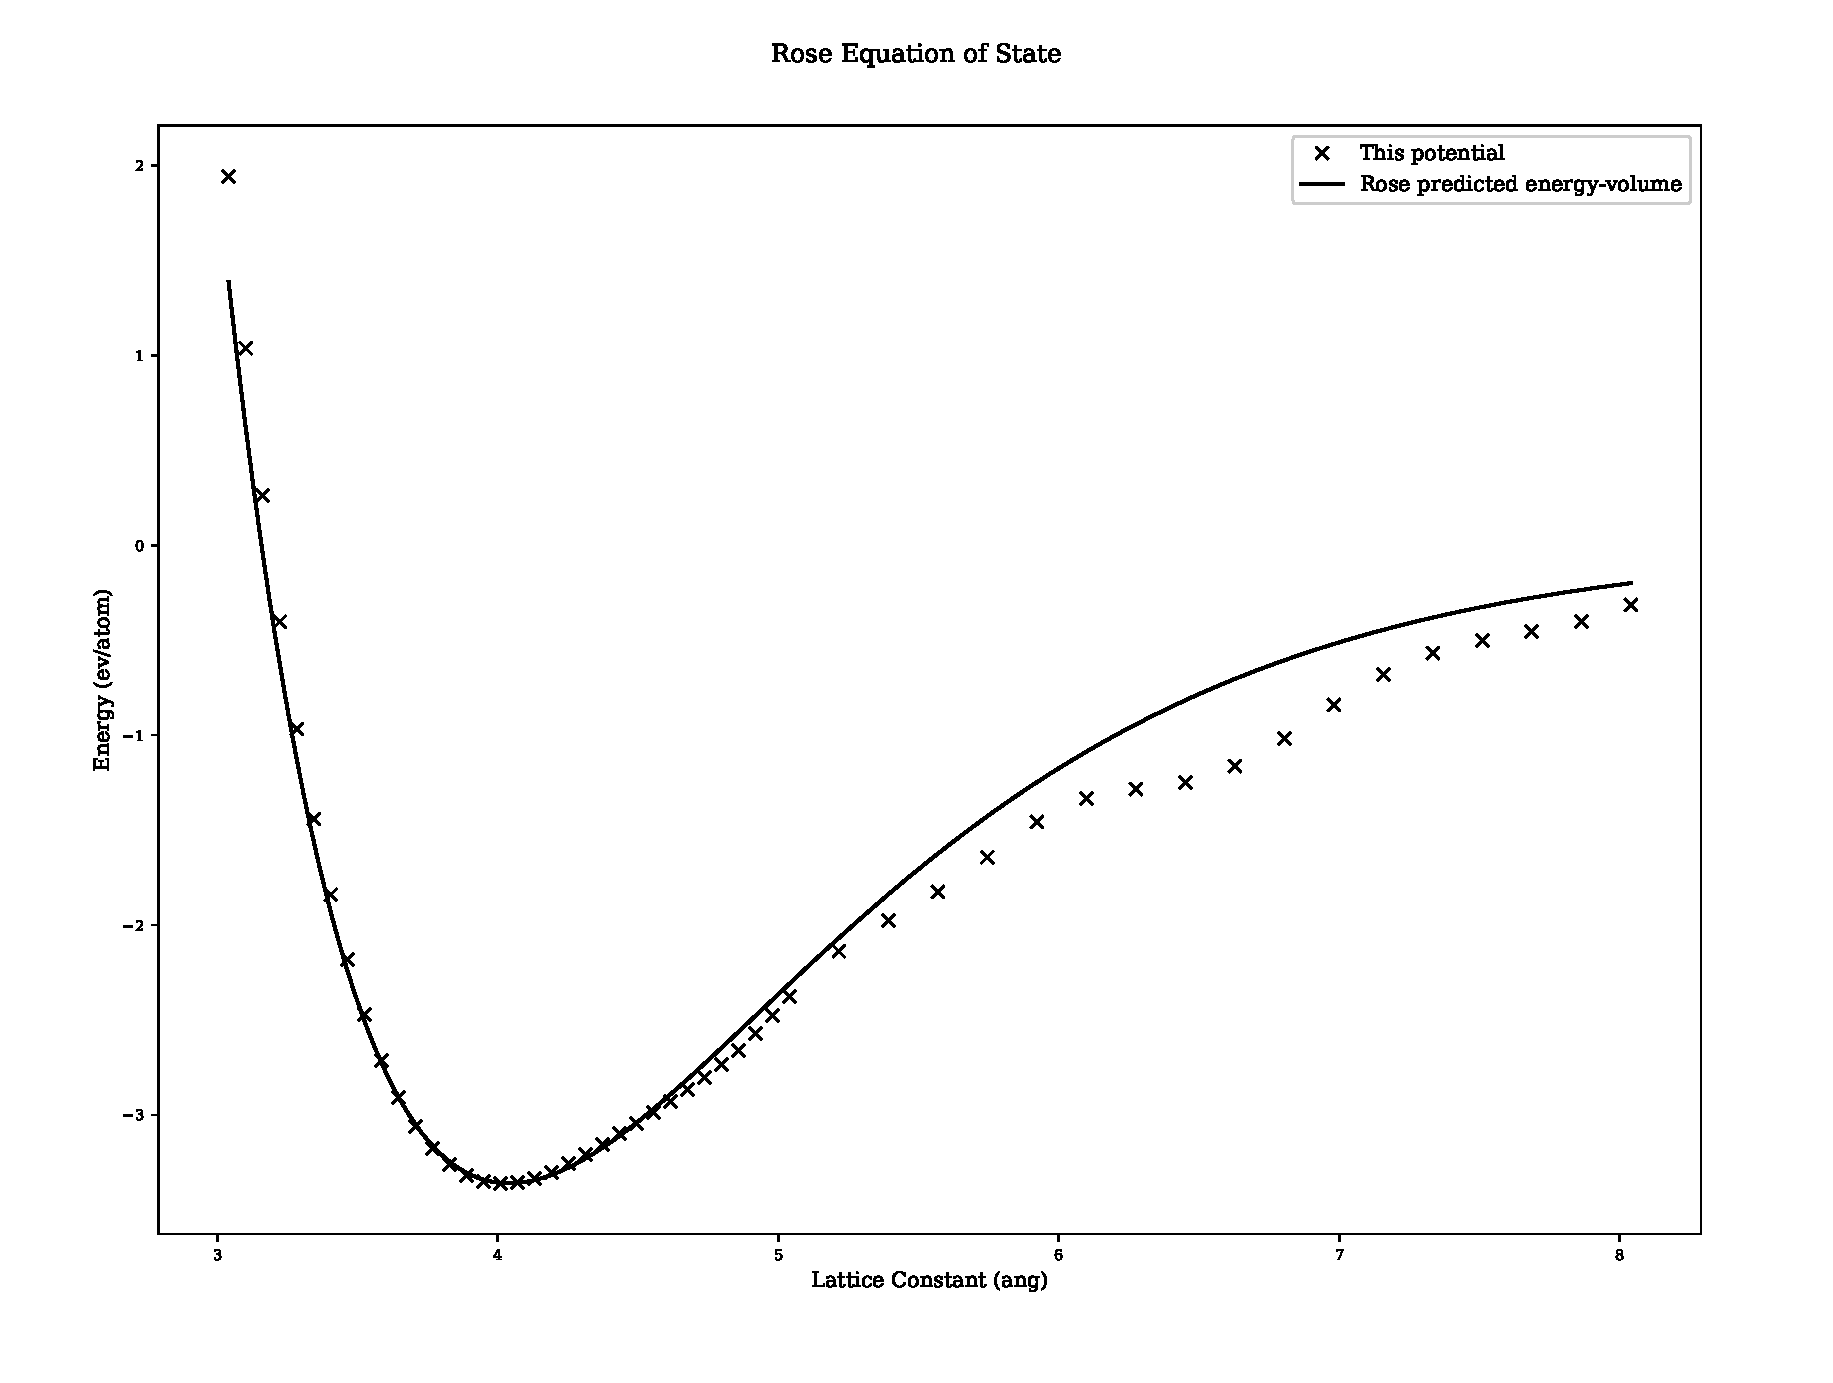
\includegraphics[width=0.6\linewidth]{appendix/transferability/transferability/Al_sheng/rose_plot_bp_fcc.eps}
  \end{center}
	\caption{Rose-Vinet equation of state for FCC Aluminium - comparison of experimental data to the Sheng Al potential}
	\label{fig:shengalfccbm}
\end{figure}

\FloatBarrier
\subsection{BCC Structure}

\begin{figure}
  \begin{center}
    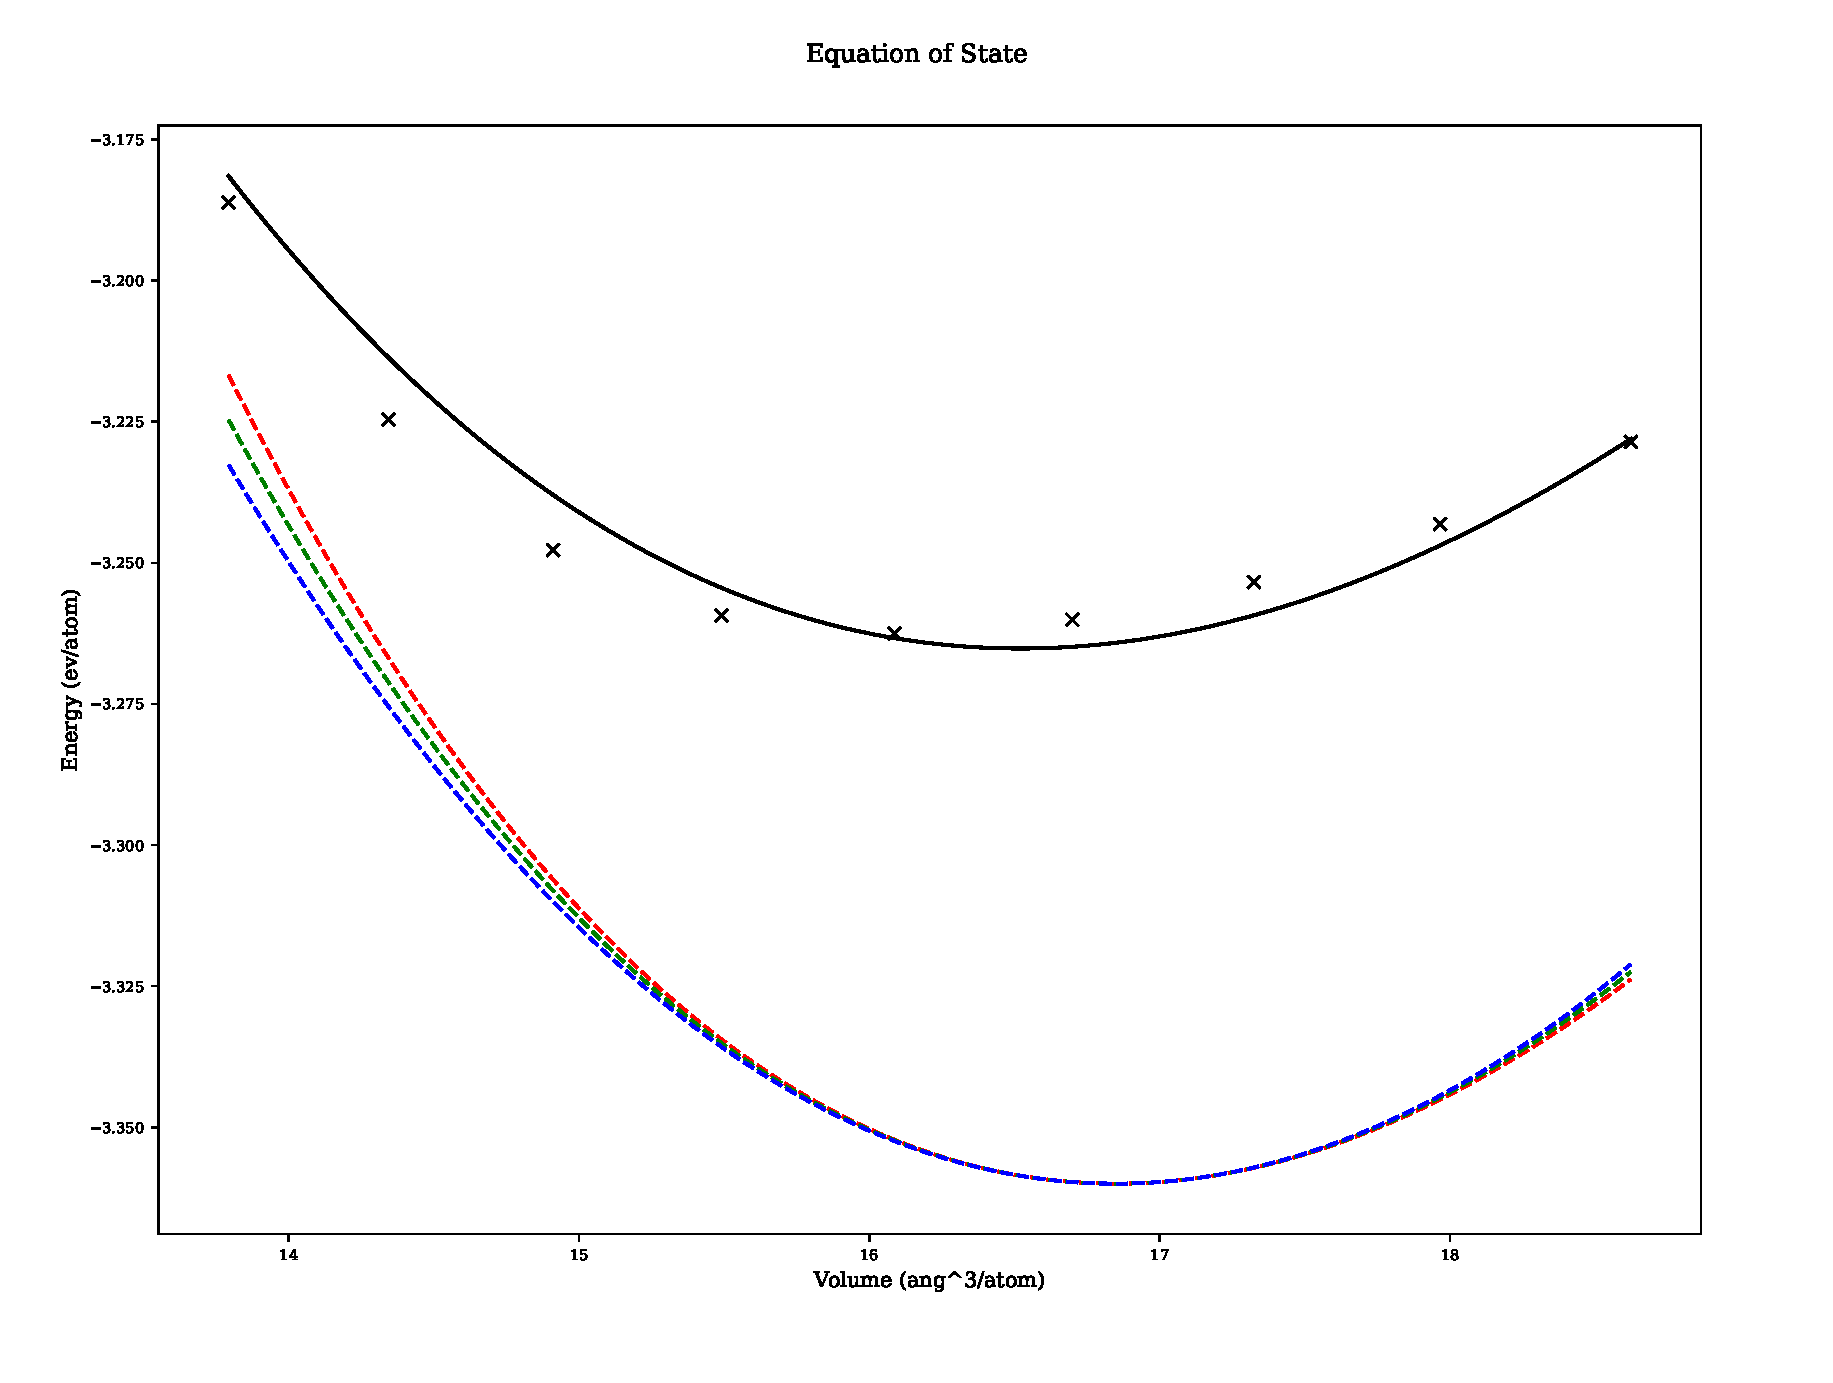
\includegraphics[width=0.6\linewidth]{appendix/transferability/transferability/Al_sheng/equation_of_state_bp_bcc.eps}
  \end{center}
	\caption{Birch Murnaghan equation of state for BCC Aluminium - comparison of experimental data to the Sheng Al potential}
	\label{fig:shengalfccbm}
\end{figure}

\begin{figure}
  \begin{center}
    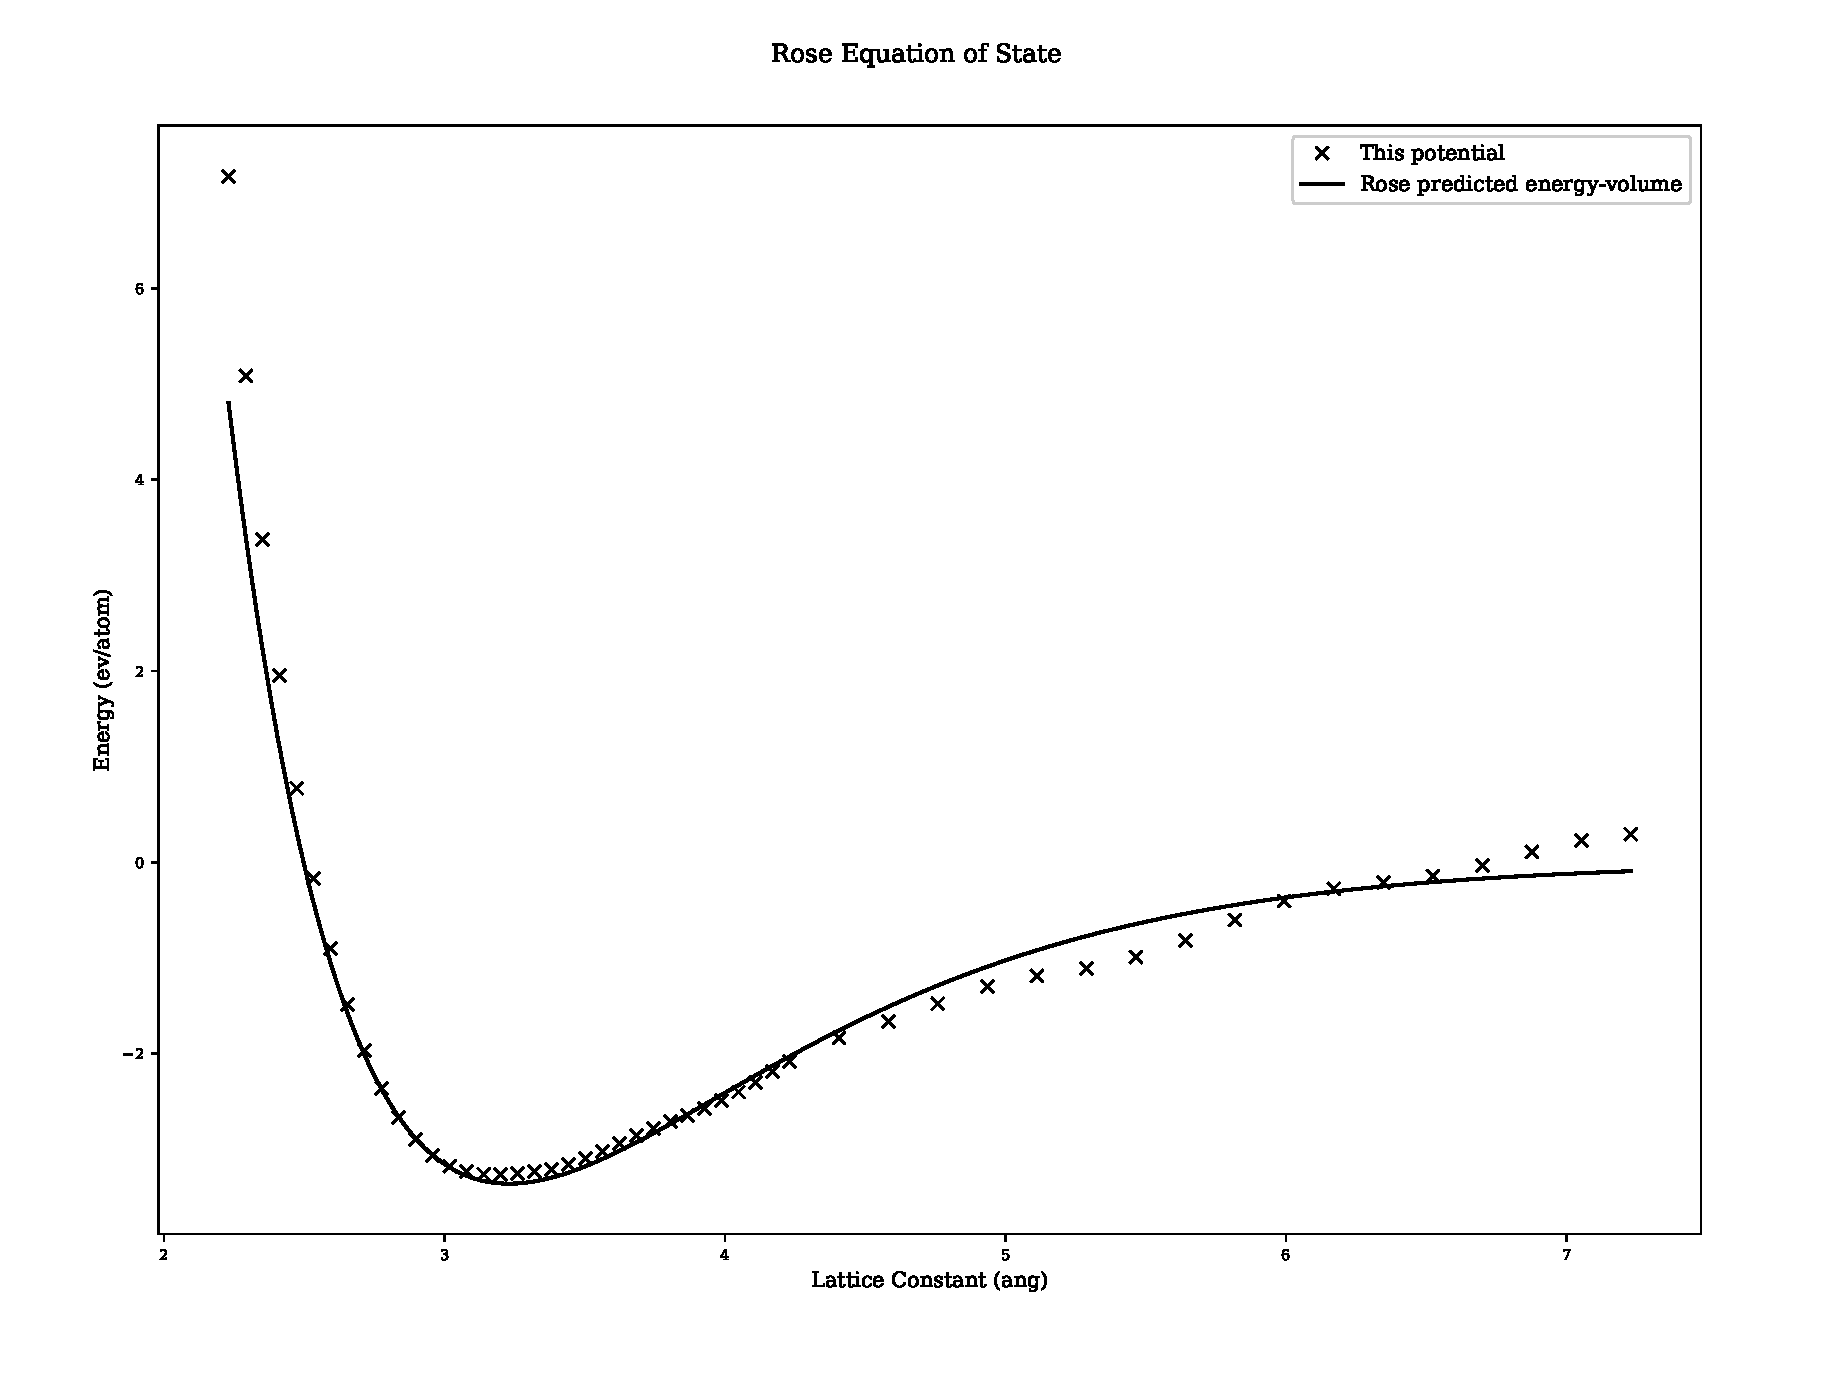
\includegraphics[width=0.6\linewidth]{appendix/transferability/transferability/Al_sheng/rose_plot_bp_bcc.eps}
  \end{center}
	\caption{Rose-Vinet equation of state for BCC Aluminium - comparison of experimental data to the Sheng Al potential}
	\label{fig:shengalfccbm}
\end{figure}









\section{Mendelev et al 2003 Iron Potential}

The EAMPA code was used to compute both the Birch-Murnaghan and Rose-Vinet equations of state using the known values for Aluminium and the Sheng Al potential\cite{femendelev}.  

\subsection{BCC Structure}
 
\begin{figure}
  \begin{center}
    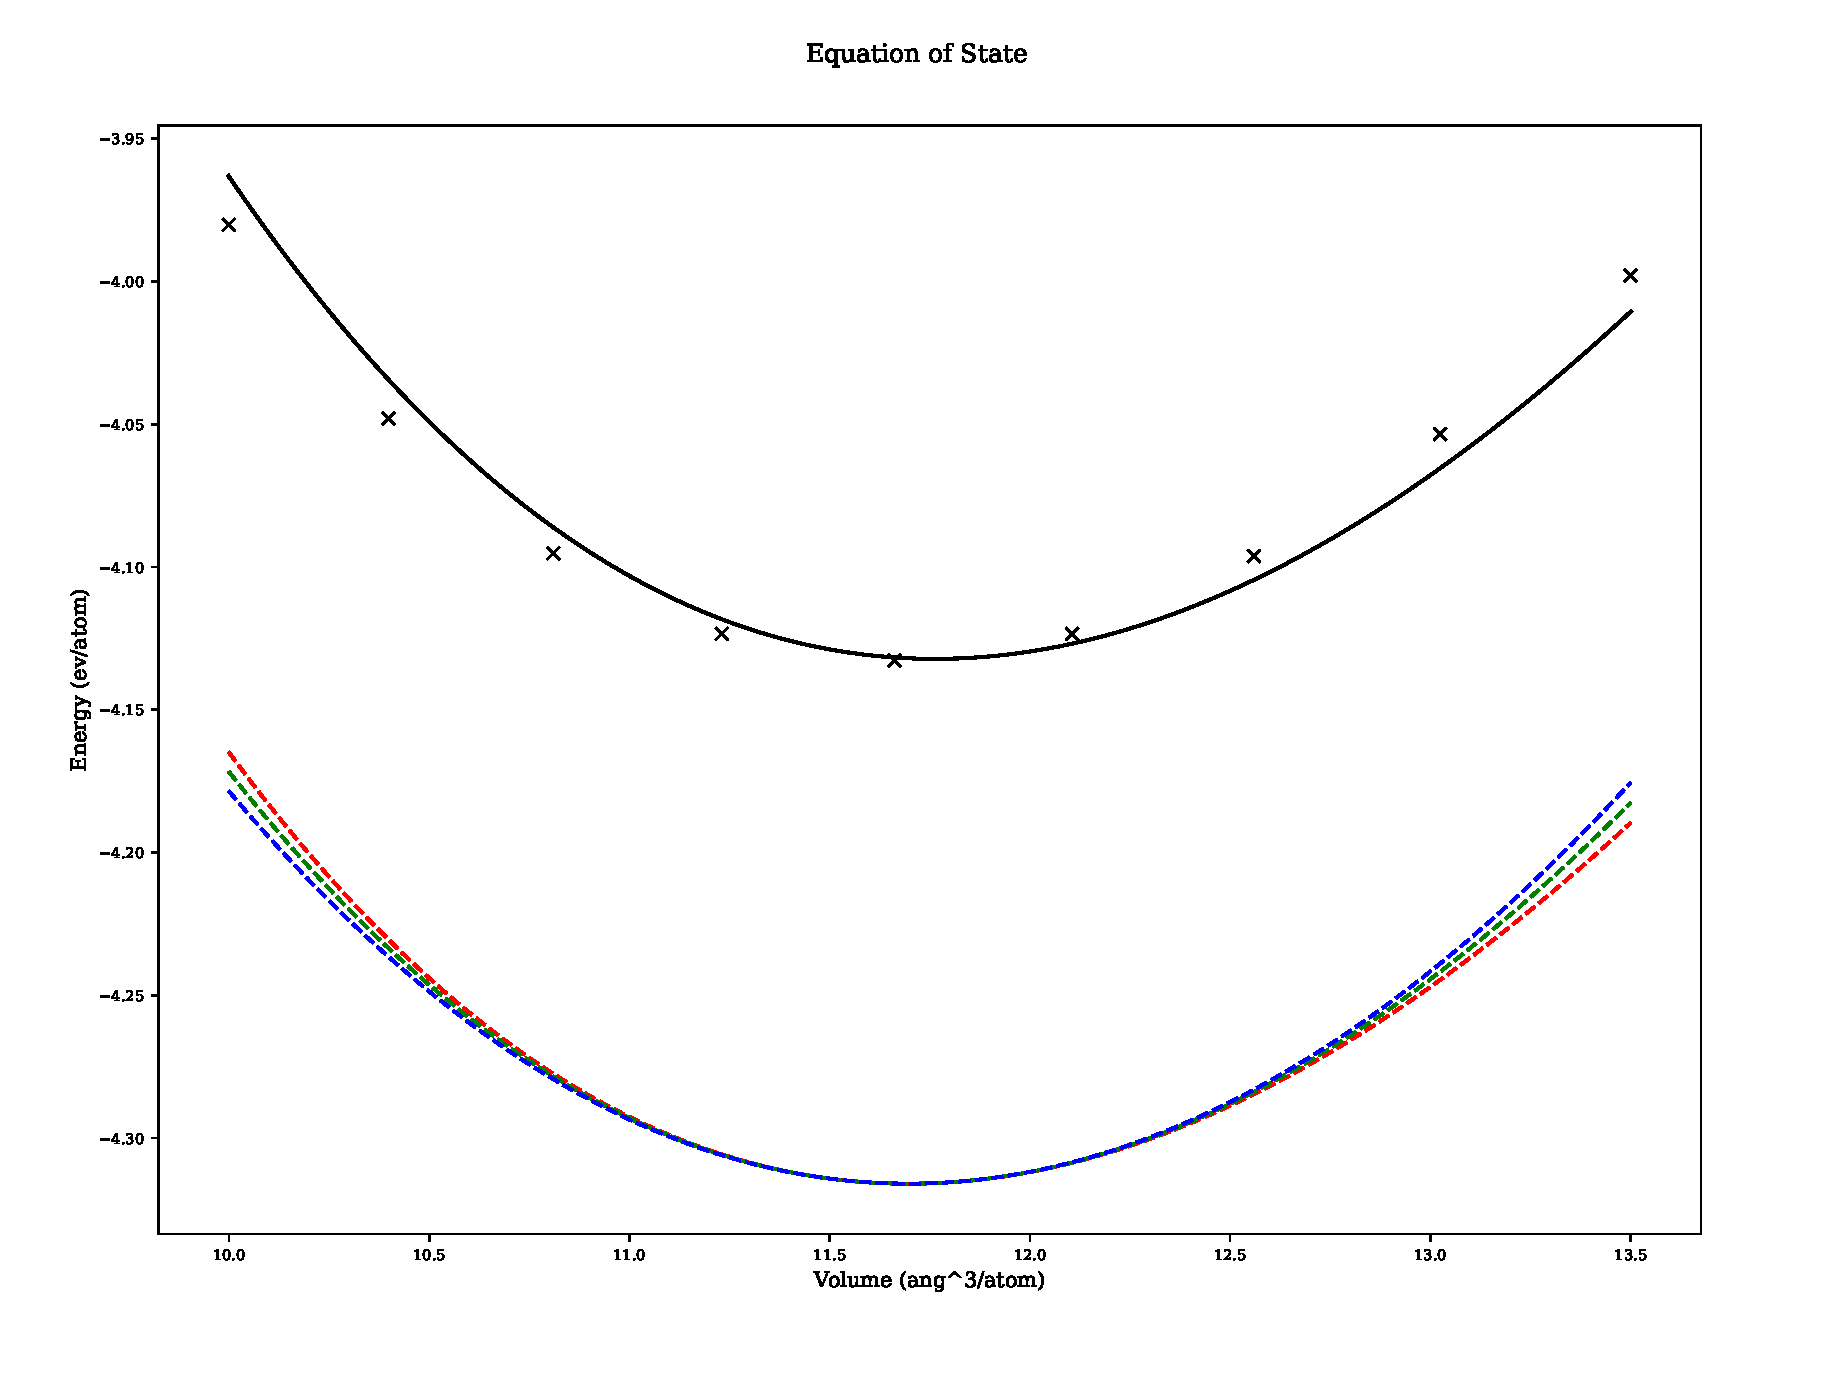
\includegraphics[width=0.6\linewidth]{appendix/transferability/transferability/Fe_mhsasa/equation_of_state_bp_bcc.eps}
  \end{center}
	\caption{Birch Murnaghan equation of state for FCC Aluminium - comparison of experimental data to the Sheng Al potential}
	\label{fig:shengalfccbm}
\end{figure}

\begin{figure}
  \begin{center}
    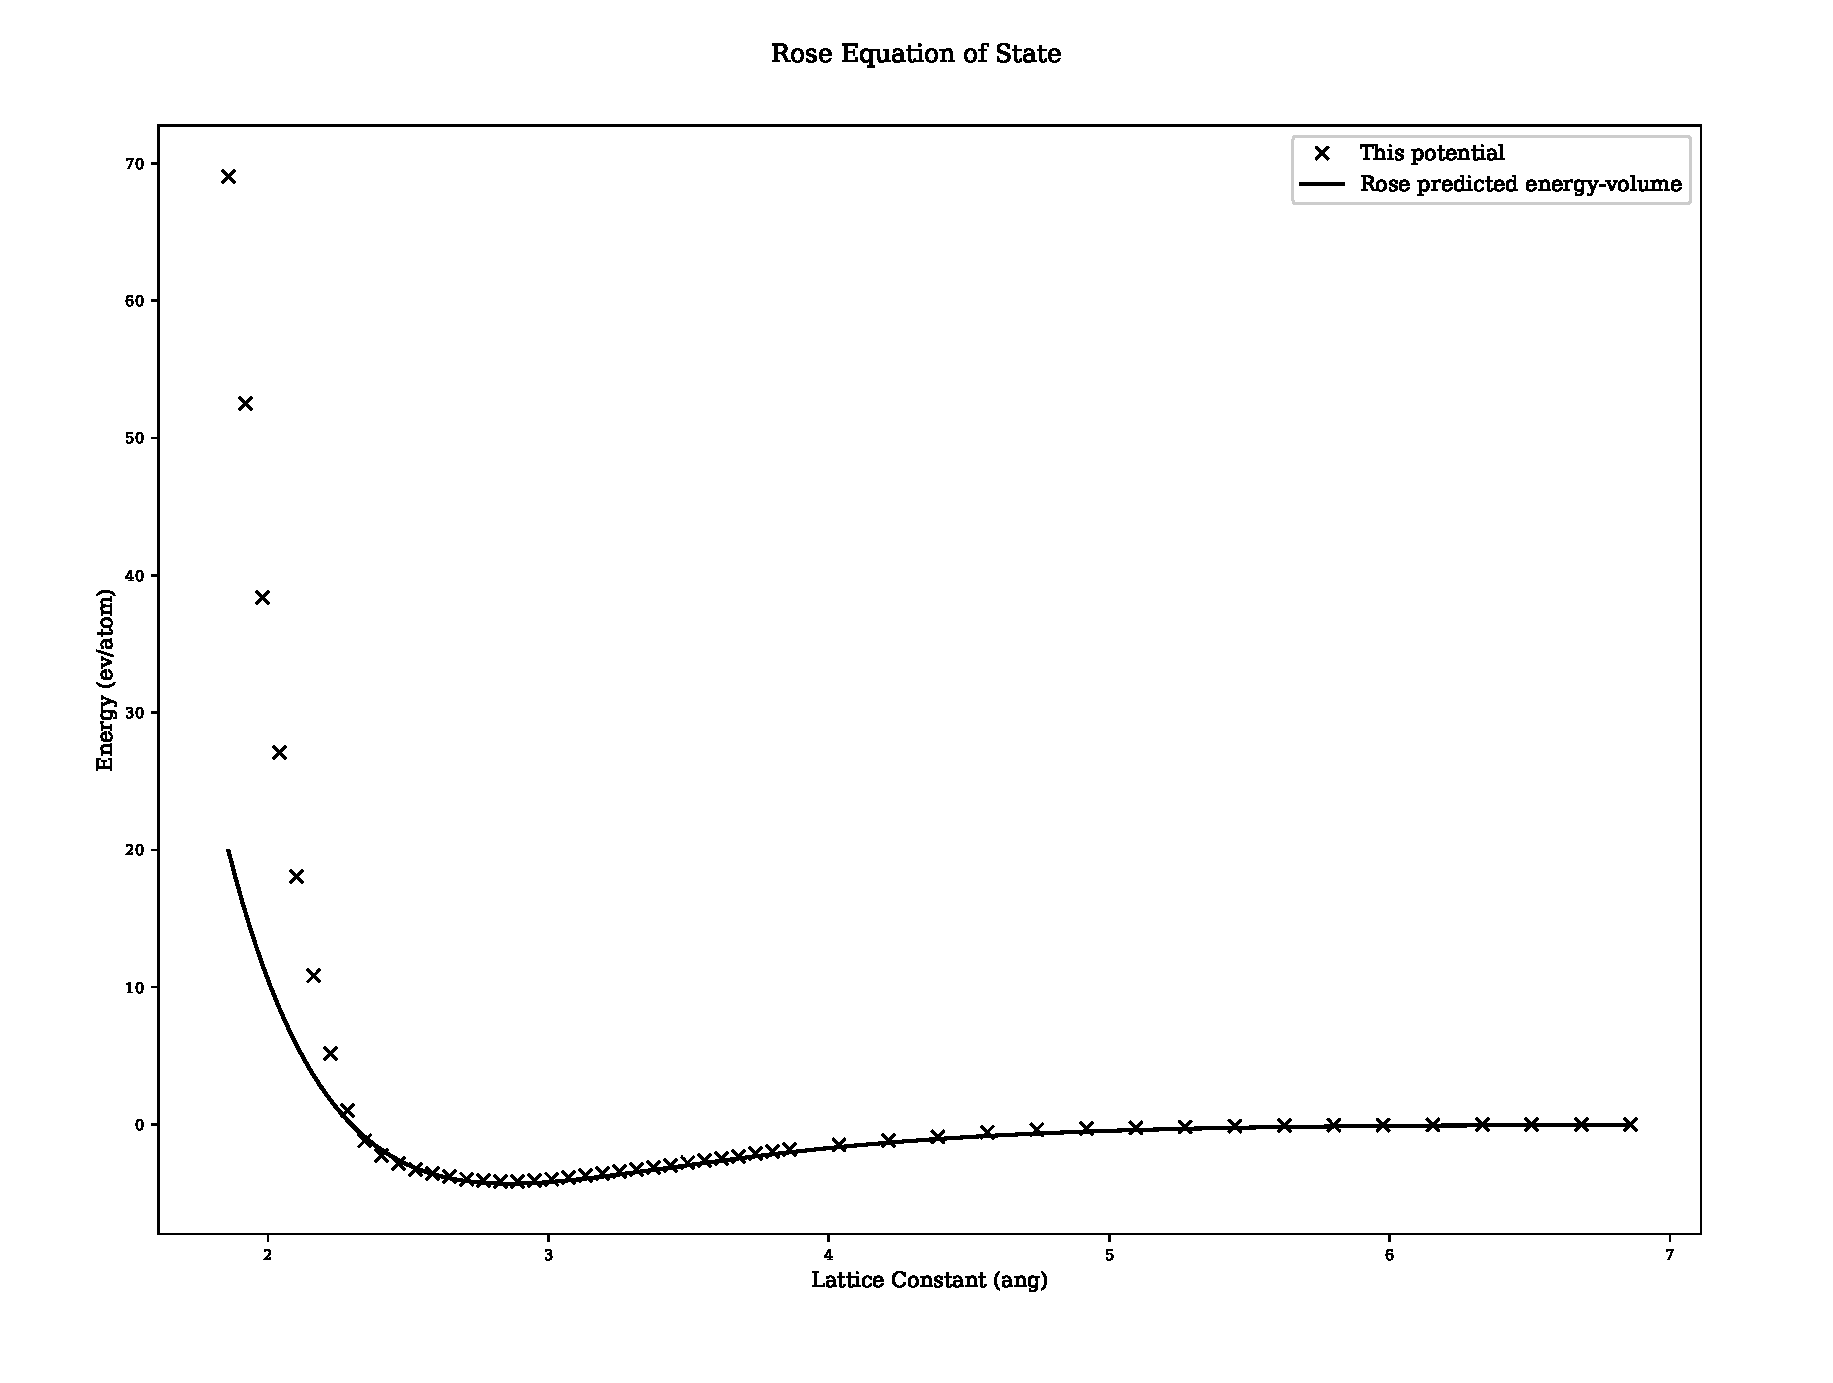
\includegraphics[width=0.6\linewidth]{appendix/transferability/transferability/Fe_mhsasa/rose_plot_bp_bcc.eps}
  \end{center}
	\caption{Rose-Vinet equation of state for FCC Aluminium - comparison of experimental data to the Sheng Al potential}
	\label{fig:shengalfccbm}
\end{figure}

\subsection{FCC Structure}
 
\begin{figure}
  \begin{center}
    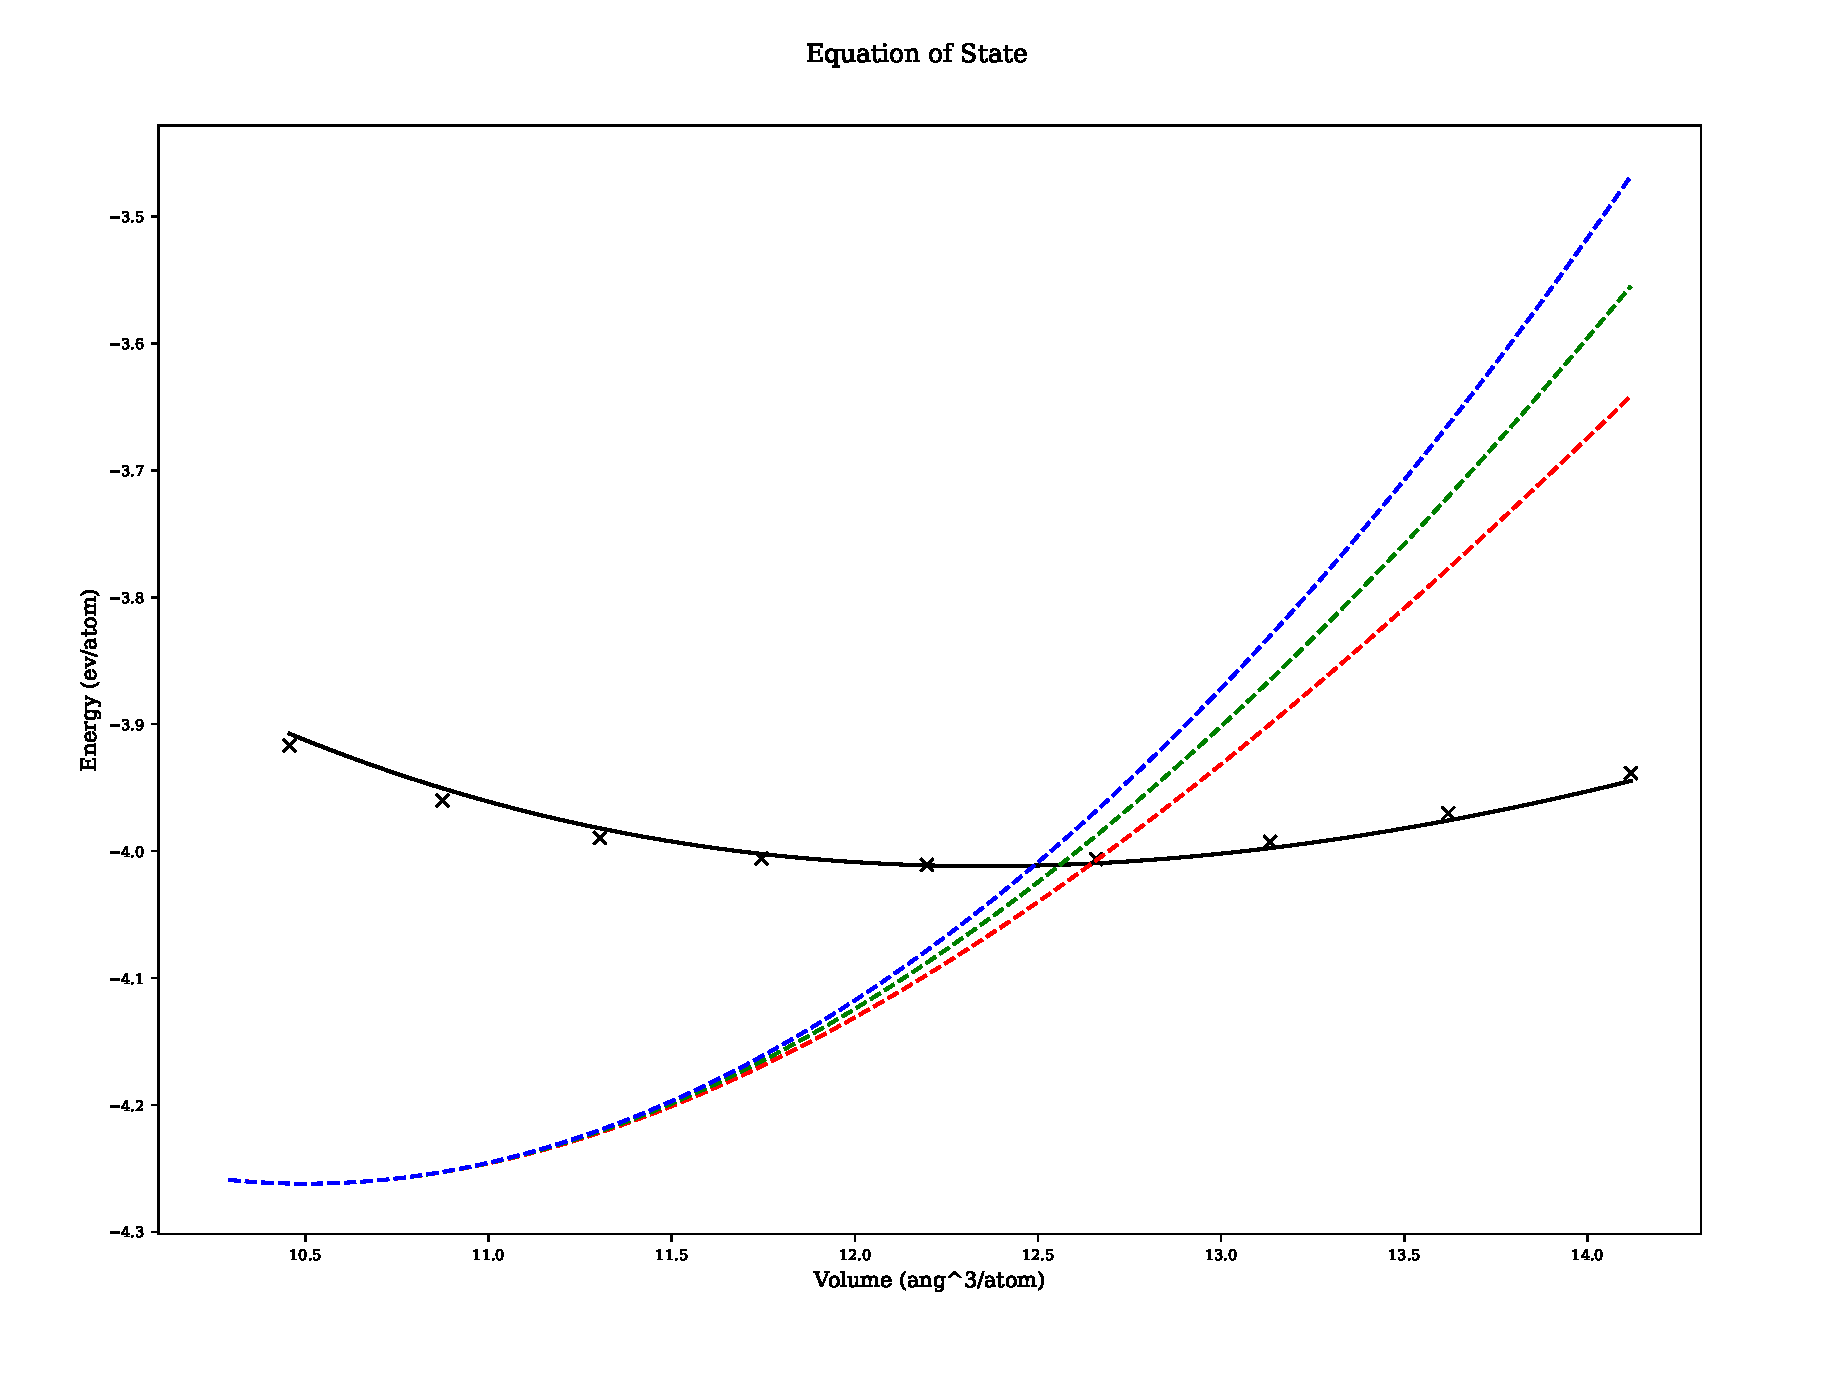
\includegraphics[width=0.6\linewidth]{appendix/transferability/transferability/Fe_mhsasa/equation_of_state_bp_fcc.eps}
  \end{center}
	\caption{Birch Murnaghan equation of state for FCC Aluminium - comparison of experimental data to the Sheng Al potential}
	\label{fig:shengalfccbm}
\end{figure}

\begin{figure}
  \begin{center}
    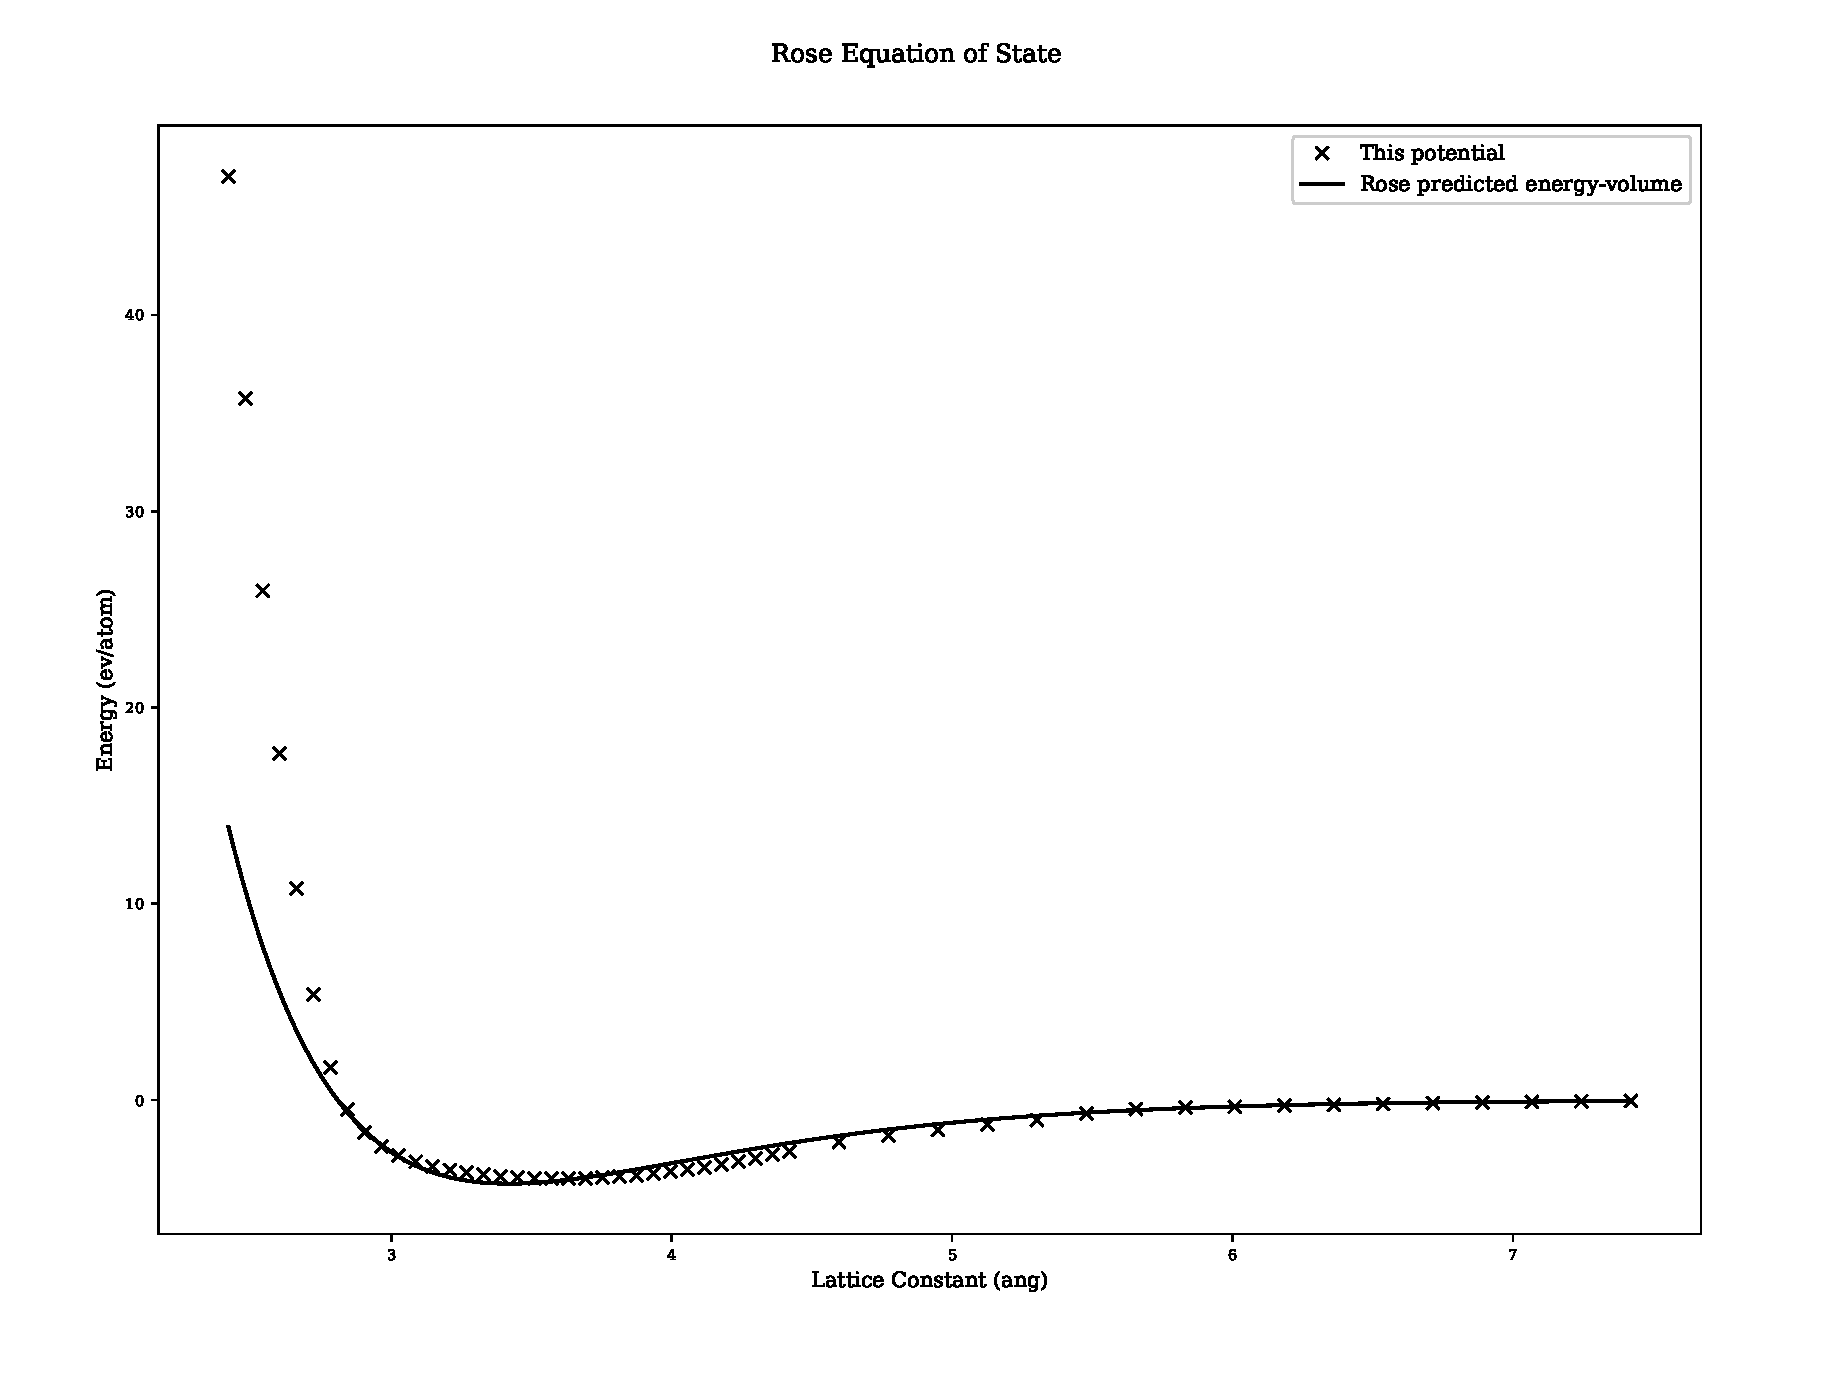
\includegraphics[width=0.6\linewidth]{appendix/transferability/transferability/Fe_mhsasa/rose_plot_bp_fcc.eps}
  \end{center}
	\caption{Rose-Vinet equation of state for FCC Aluminium - comparison of experimental data to the Sheng Al potential}
	\label{fig:shengalfccbm}
\end{figure}








\section{Ackland et al 1997 Iron Potential}

The EAMPA code was used to compute both the Birch-Murnaghan and Rose-Vinet equations of state using the known values for Aluminium and the Sheng Al potential\cite{Fe_abch}.  

\subsection{BCC Structure}
 
\begin{figure}
  \begin{center}
    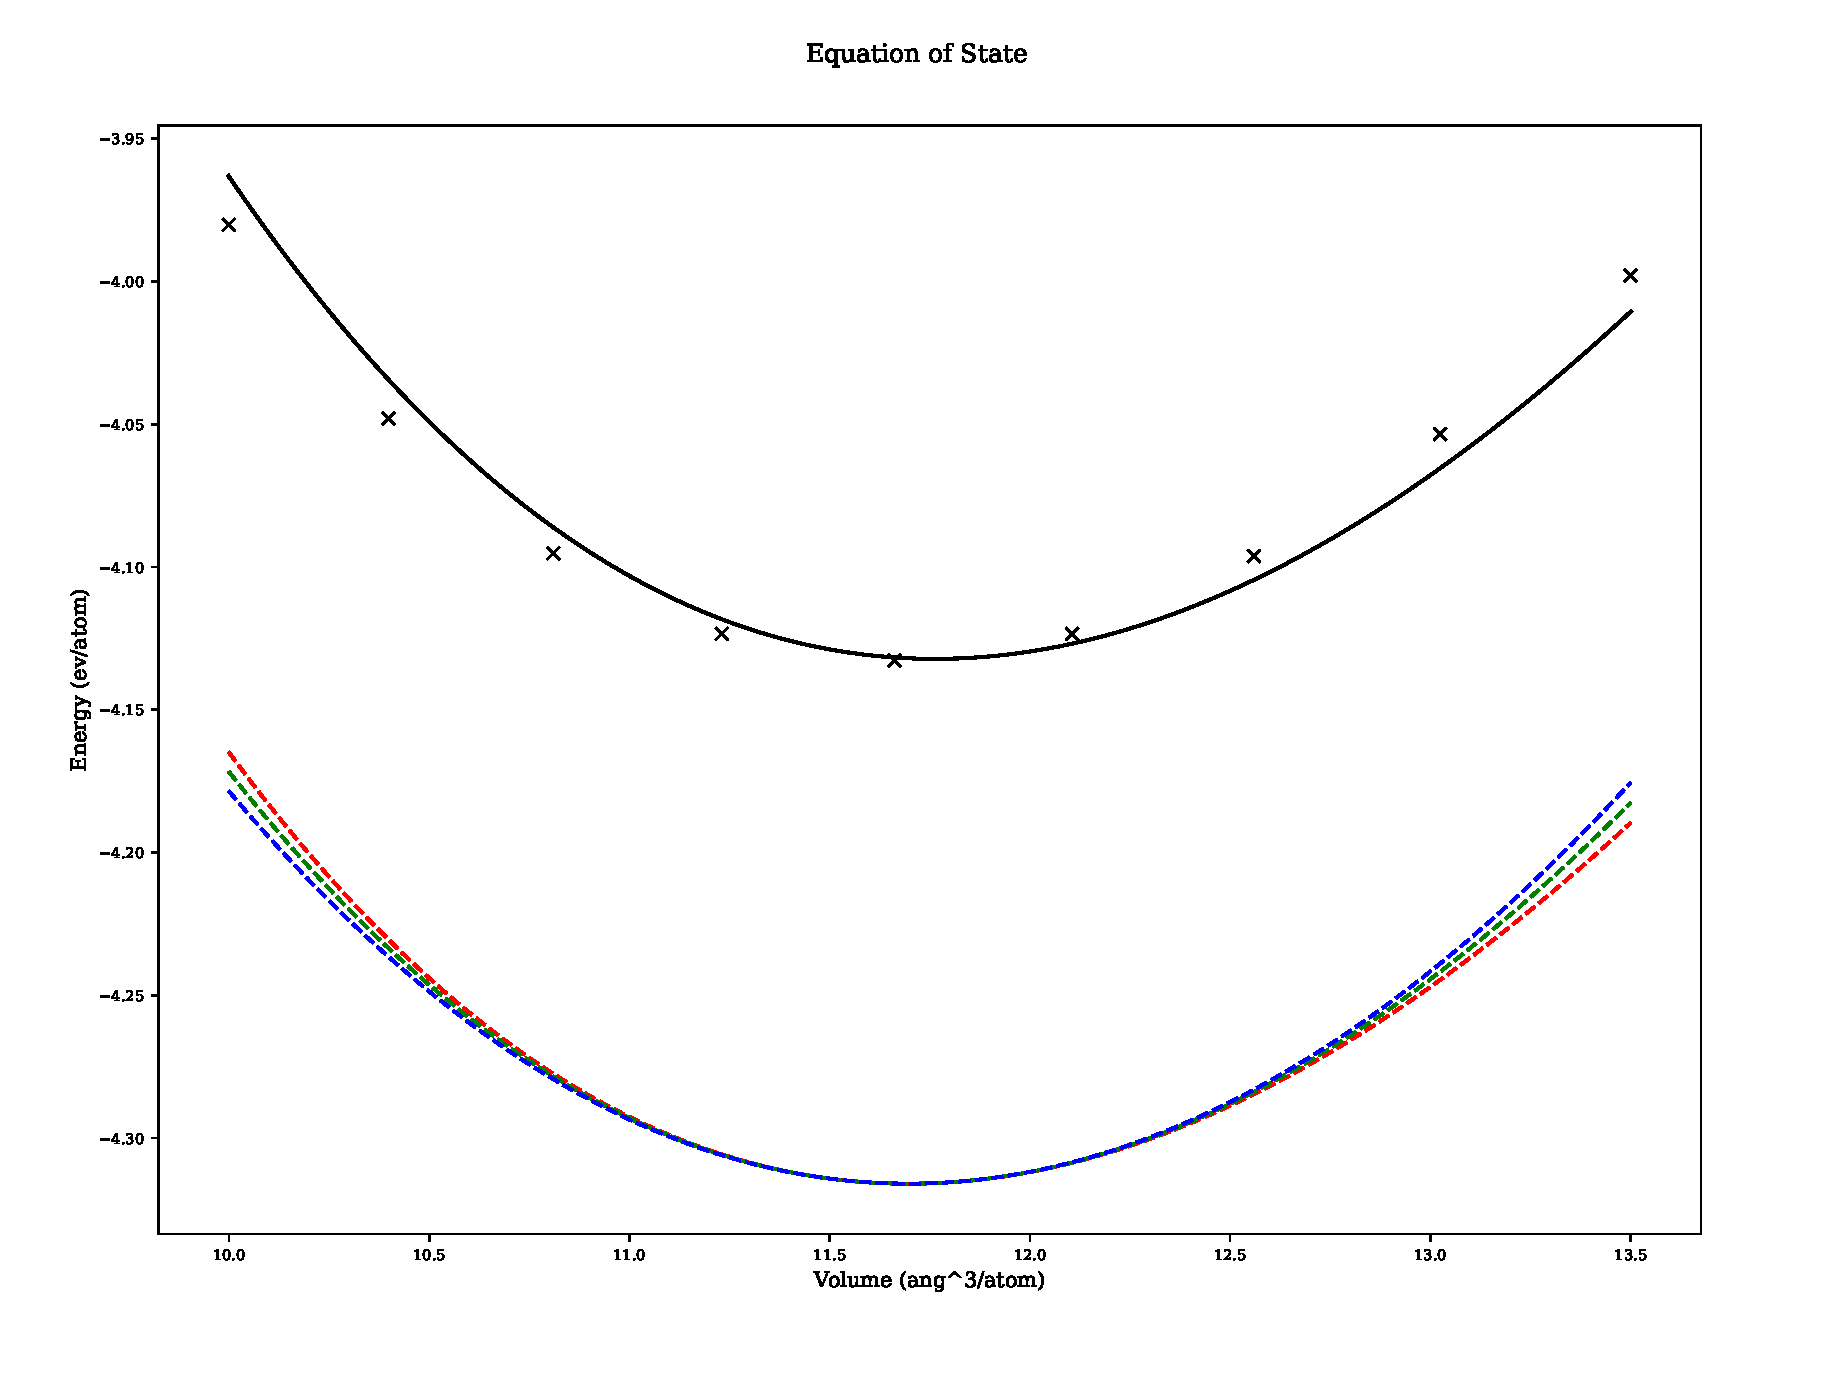
\includegraphics[width=0.6\linewidth]{appendix/transferability/transferability/Fe_mhsasa/equation_of_state_bp_bcc.eps}
  \end{center}
	\caption{Birch Murnaghan equation of state for FCC Aluminium - comparison of experimental data to the Sheng Al potential}
	\label{fig:shengalfccbm}
\end{figure}

\begin{figure}
  \begin{center}
    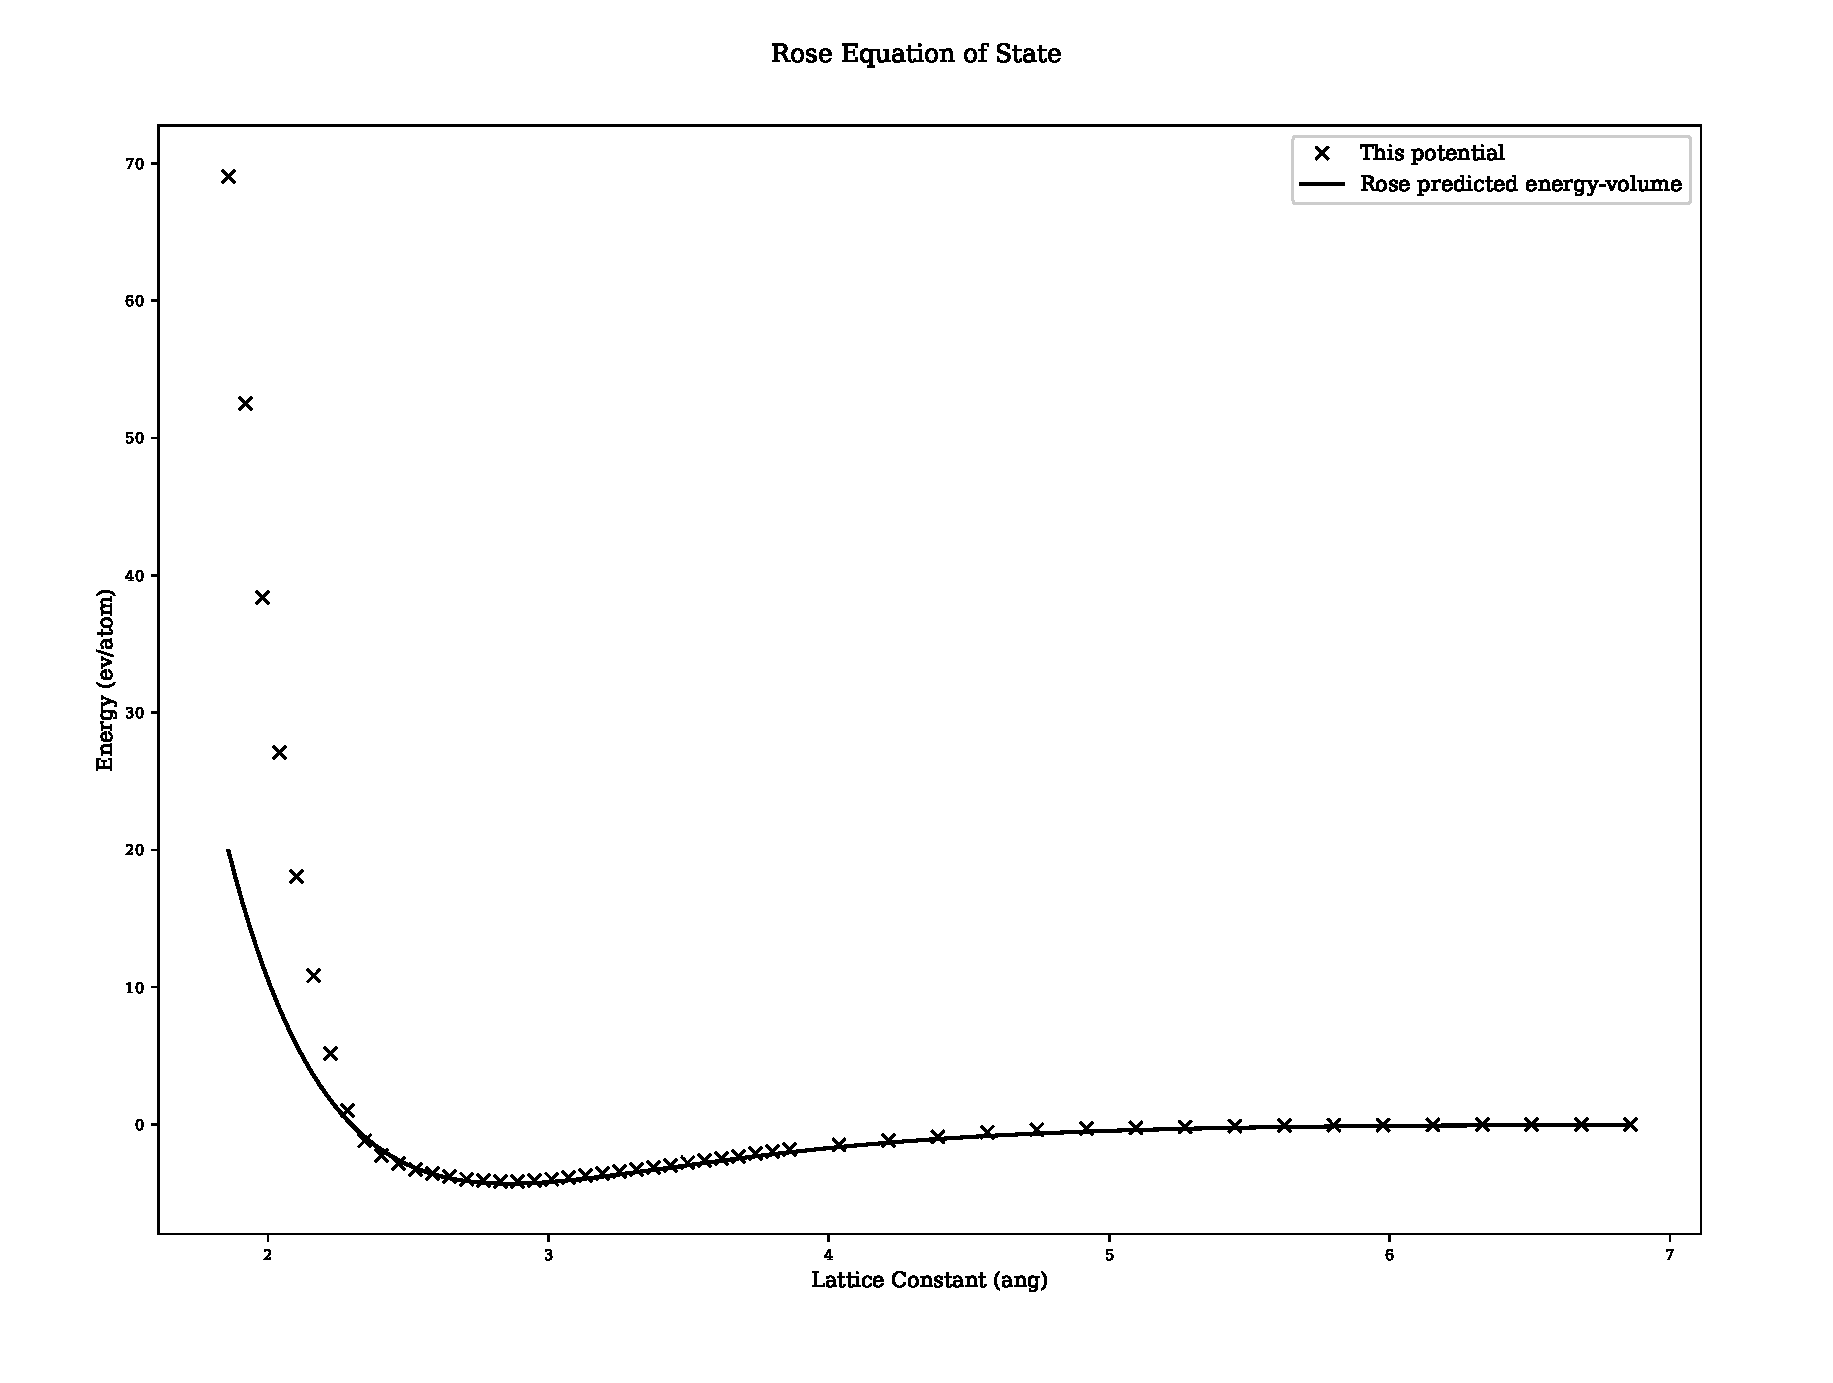
\includegraphics[width=0.6\linewidth]{appendix/transferability/transferability/Fe_mhsasa/rose_plot_bp_bcc.eps}
  \end{center}
	\caption{Rose-Vinet equation of state for FCC Aluminium - comparison of experimental data to the Sheng Al potential}
	\label{fig:shengalfccbm}
\end{figure}

\subsection{FCC Structure}

The EAMPA code was used to compute both the Birch-Murnaghan and Rose-Vinet equations of state using the known values for Aluminium and the Sheng Al potential\cite{shengeamonline}.  
 
\begin{figure}
  \begin{center}
    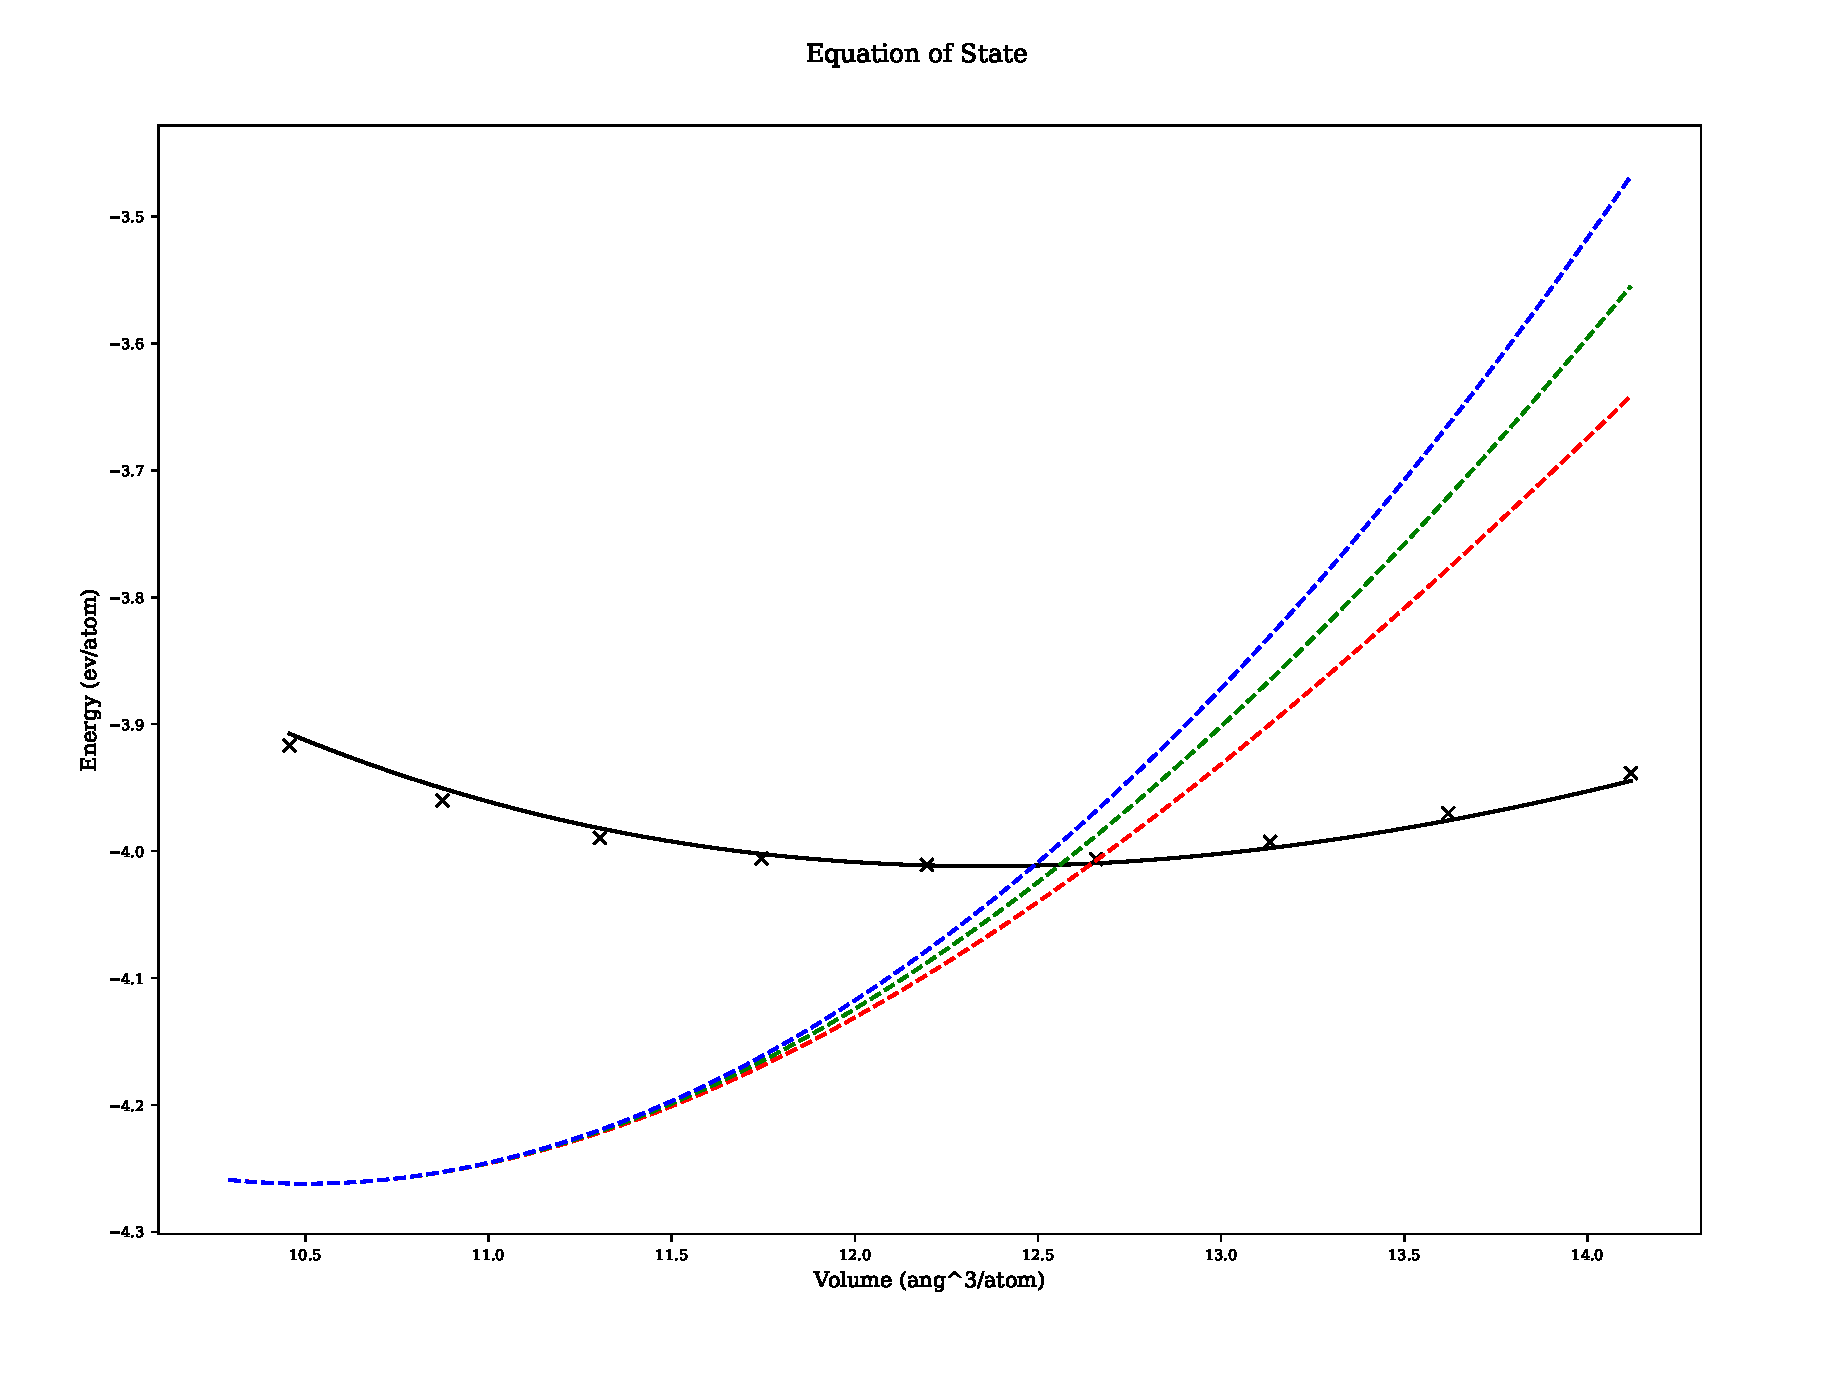
\includegraphics[width=0.6\linewidth]{appendix/transferability/transferability/Fe_mhsasa/equation_of_state_bp_fcc.eps}
  \end{center}
	\caption{Birch Murnaghan equation of state for FCC Aluminium - comparison of experimental data to the Sheng Al potential}
	\label{fig:shengalfccbm}
\end{figure}

\begin{figure}
  \begin{center}
    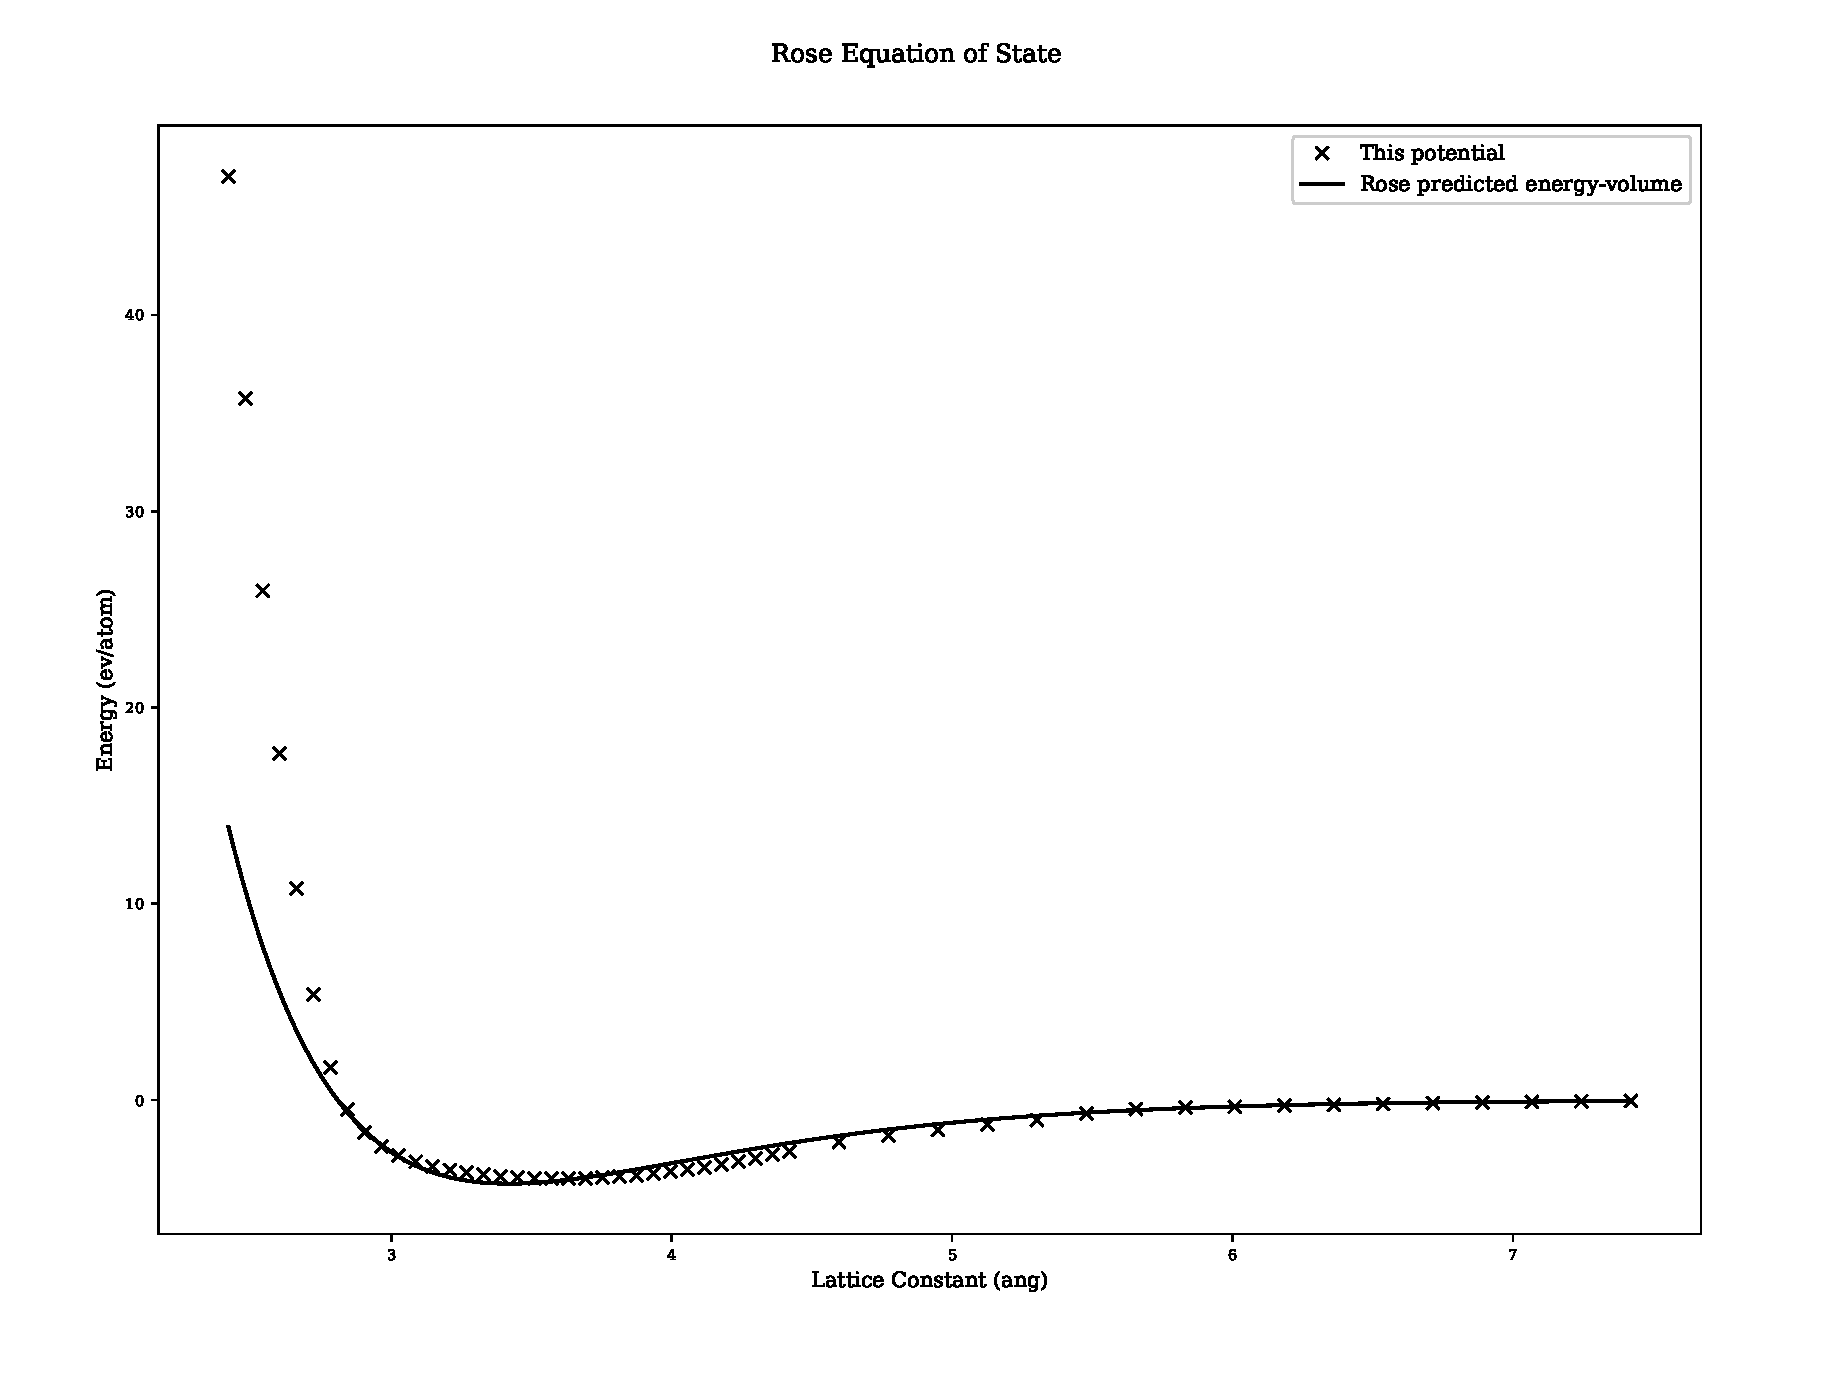
\includegraphics[width=0.6\linewidth]{appendix/transferability/transferability/Fe_mhsasa/rose_plot_bp_fcc.eps}
  \end{center}
	\caption{Rose-Vinet equation of state for FCC Aluminium - comparison of experimental data to the Sheng Al potential}
	\label{fig:shengalfccbm}
\end{figure}















